\section{Data}\label{sec:data}

In this thesis, we will work with data from the ${}^{46}Ar(p, p')$ experiment conducted at the national superconducting cyclotron laboratory (NSCL) located on the Michigan state university campus. We principally work with two different data sources: data from AT-TPC simulation tools, and data recorded in the AT-TPC experiment proper. The experimental data were recorded from a single run of the experiment, which yields on the order of $\sim 10^4$ events.    For the simulated data, we construct two datasets on the order of $\sim10^3$ and $\sim10^4$ events, respectively. In this section we give a brief overview of the data, for a more in-depth consideration we refer to \cite{Mittig2015}, \cite{Suzuki2012} and  \cite{Bradt2017a}. 

In this thesis we will explore the machine learning algorithms described in chapters \ref{ch:ml} and \ref{ch:autoencoder} on three datasets from the AT-TPC, listed in table \ref{tab:datasets}. The simulated data will serve as a baseline for performance, while the filtered and full data are real records from the ${}^{46}Ar$ experiment. The former of which has some post-processing applied to remove noise, and the latter having no such processing applied. The details of the post-processing are given in later sections. First, we consider the pipeline from raw data to images that the algorithms described in chapter \ref{ch:autoencoder} can process. 

\begin{table}[H]
\centering
\caption{Descriptions of number of events in the data used for analysis in this thesis. In principle we can simulated infinite data, but it is both quite simple and not very interesting outside a case for a proof-of-concept}\label{tab:datasets}
\begin{tabular}{lccc}
\toprule
{} & Simulated & Full & Filtered \\
\midrule
Total &  $8000$ & $51891$ & $49169$ \\
Labeled & $2400$ & $1774$ &  $1582$ \\ 
\bottomrule
\end{tabular}
\end{table}

\subsection{Data processing}

Our data processing pipeline begins with localized point-cloud data in the two-dimensional detector coordinate system, with one time dimension and a corresponding charge measurement. The charge and time measurement are extracted as the peak of this signal over the event, resulting in a maximum of one measurement per pad in the sensor plane. The events range from fairly sparse $< 10^2$ records to being very populated, depending on where in the volume the reaction occurs as well as other noise-generating factors. We centre the charge data to values $>1$ by adding the lowest occurring record in the run and apply a log-transform to get values in $\R^+$. Subsequently, we scale by the maximum value in the run to get charge data in the interval $[0, 1]$. Lastly, the transformed charge data is saved in a two-dimensional $128px\, \times \,128px$ array using the \lstinline{matplotlib} package provided in the \lstinline{Python} programing language (\cite{matplotlib}). The choice of scaling was made to accommodate a binary cross-entropy loss on a 2D projection, as it presumes the true values to be bounded as probabilities.

We will begin by considering the simulated events, followed by subsequent considerations of the full and filtered experimental data.

\subsection{Simulated \texorpdfstring{${}^{46}Ar$}{46Ar}  events}\label{sec:data_sim}

The simulated AT-TPC tracks were simulated with the \lstinline{pytpc} package developed by \citet{Bradt2017a}. Using the same parameters as for the $Ar^{46}(p, p)$ experiment, a small set of $N=4000$ events were generated per class, as well as a larger set of $N=40000$ events per class. The events are generated as point-clouds, consisting of position data on the x-y plane, a time-stamp and an associated charge value. These point-clouds are transformed into pure x-y projections with charge intensity for the analysis in this thesis using the pipeline described in the previous section. 

More formally the events are originally composed of peak-only 4-tuples of $e_i = (x_i, y_i, t_i, c_i)$. The peak-only designation indicates that we use the recorded peak amplitude on each pad, the tuples then correspond to pads that recorded a signal for that event. Each event is then a set of these four-tuples: $\epsilon_j = \{e_i\}$ creating a track in three-dimensional space. 

To emulate the real-data case, we set a subset of the simulated data to be labelled and treat the rest as unlabeled data. We chose this partition to be $15\%$ of each class. We denote this subset and its associated labels as $\gamma_L=(\mathbf{X}_L, \mathbf{y}_L)$, the entire dataset which we will denote as $\mathbf{X}_F$. To clarify, please note that $\mathbf{X}_L \subset \mathbf{X}_F$.

We display two simulated events in figure \ref{fig:sim_samples}. The top row illustrates a proton-event, and the bottom a carbon-event. 

\begin{figure}[H]
\centering
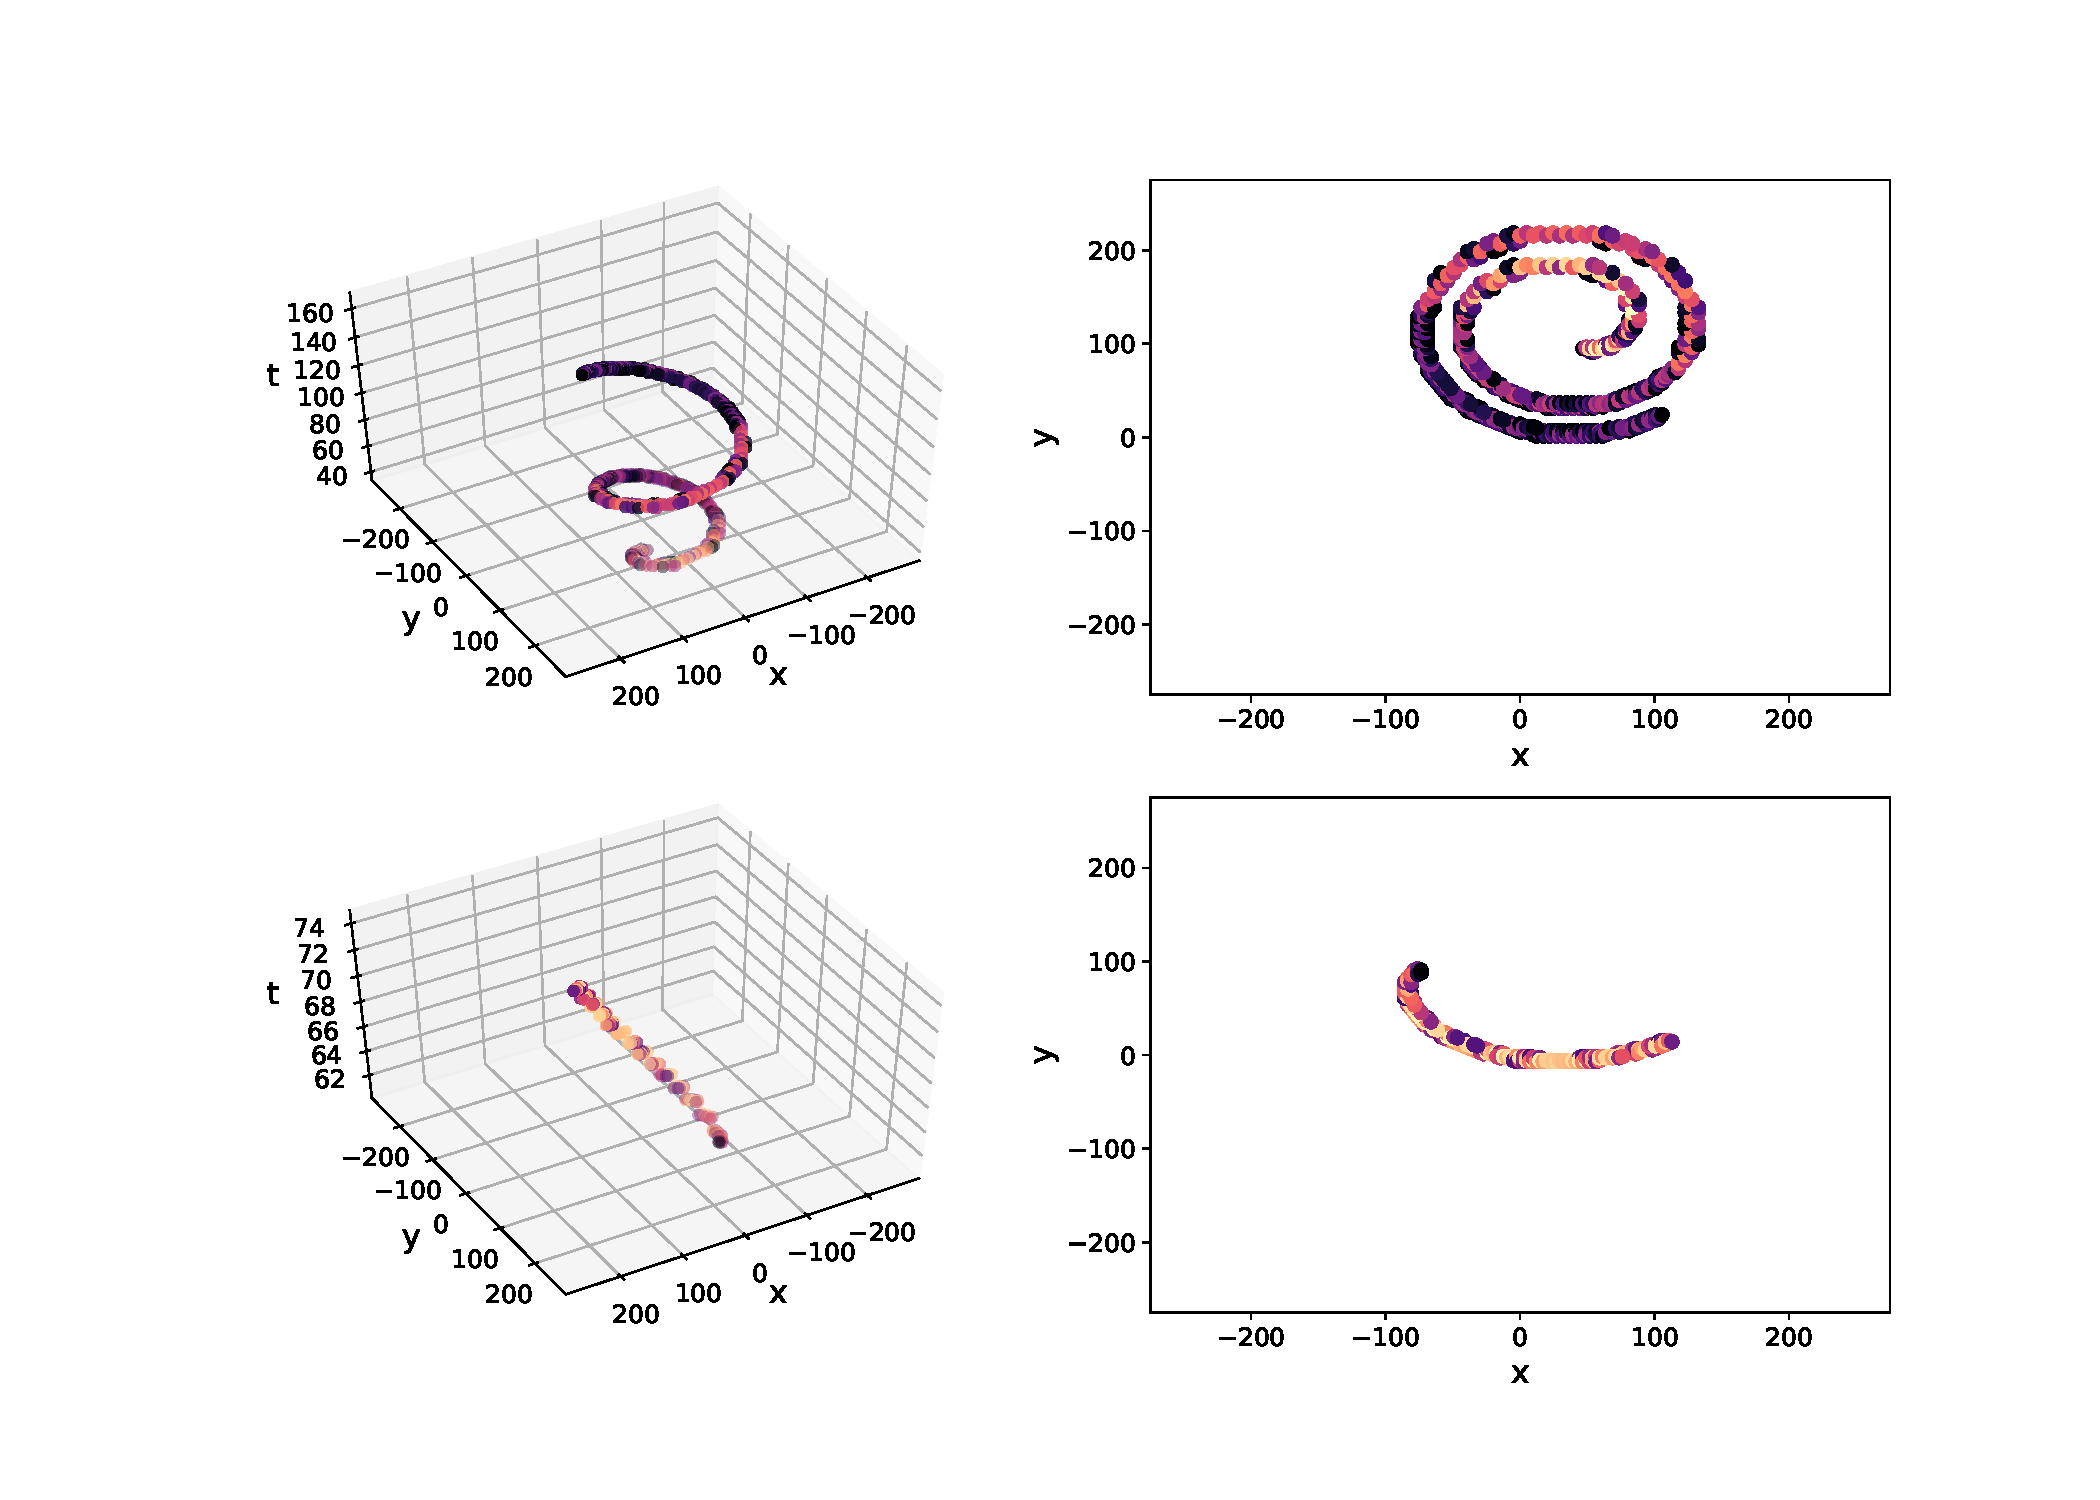
\includegraphics[width=\textwidth]{../plots/display_eventssimulated.pdf}
\caption[Displaying simulated events in 2D and 3D]{Two- and three-dimensional representations of two events from a simulated ${}^{46}Ar$ experiment. Each row is one event in two projections, where the lightness of each point indicates higher charge values.}\label{fig:sim_samples}
\end{figure}


\subsection{Full \texorpdfstring{${}^{46}Ar$}{46Ar}  events}\label{sec:data_real}

The events analyzed in this section were retrieved from the ${}^{46}Ar$ resonant proton scattering experiment recorded with the AT-TPC. 

The sensor plane in the AT-TPC is very sensitive, as such there is substantial noise in the ${}^{46}Ar$ data. The noise can be attributed to structural noise from electronics cross-talk, and possible interactions with cosmic background radiation, as well as other sources of charged particles. Part of the challenge for this data then comes from understanding of the physics of the major contributing factors to this noise. 

We display two different events from the ${}^{46}Ar$ experiment in figure \ref{fig:samples}. The top row illustrates an event with a large fraction of noise, while the bottom row shows an event nearly devoid of noise. The very clear spiral structure of the bottom row indicates that this is a proton-event.

\begin{figure}[H]
\centering
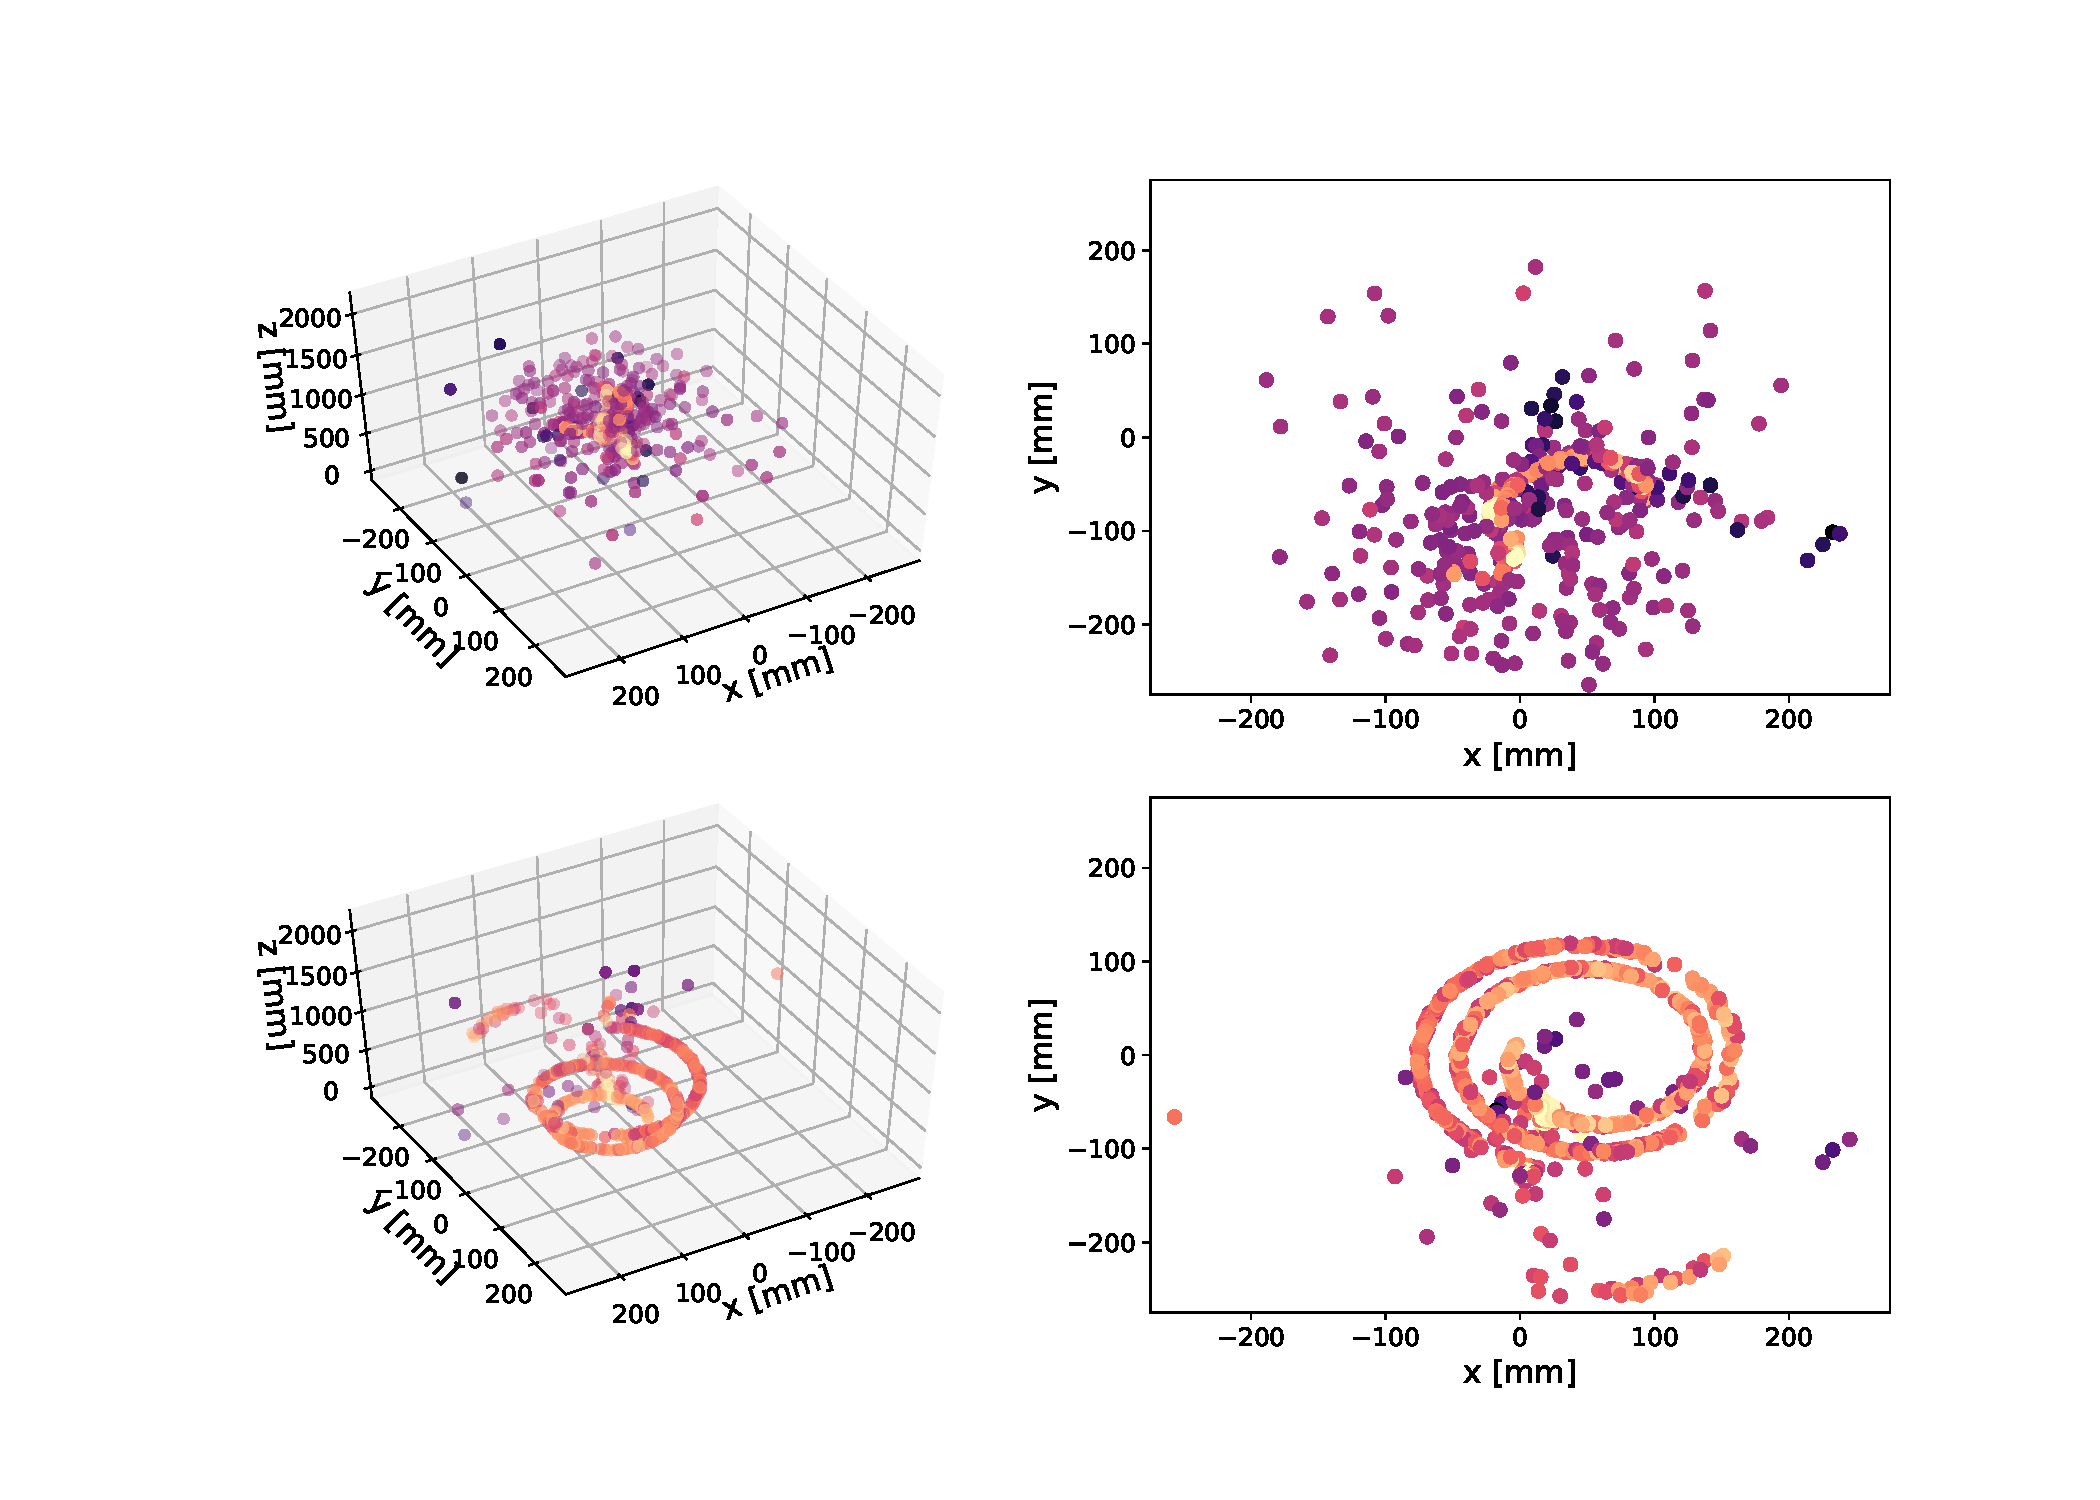
\includegraphics[width=\textwidth]{../plots/display_eventsfull_.pdf}
\caption[Displaying un-filtered events in 2D and 3D]{Two- and three-dimensional representations of two events from the ${}^{46}Ar$ experiment. Each row is one event in two projections, where the lightness of each point indicates higher charge values.}\label{fig:samples}
\end{figure}

\subsection{Filtered \texorpdfstring{${}^{46}Ar$}{46Ar} events}\label{sec:filtered}

As we saw in the previous section, the detector picks up a significant amount of noise. We split the noise broadly in two categories,  one being random-uncorrelated noise and the second is structured noise. The former can be quite trivially removed with a nearest-neighbour algorithm that checks if a point in the event is close to any other. To remove the correlated noise, researchers at the NSCL developed an algorithm based on Hughes' transform. This transformation is a common technique in computer vision, used to identify common geometric shapes like lines and circles. Essentially, the algorithm draws many lines (of whatever desired geometry) through each data-point and checks whether these lines intersect with points in the dataset. Locations in parameter space that generate many intersections then become bright spots, allowing us to filter away points that are not close to these points. These algorithms remove a large amount of the unstructured noise and are computationally rather cheap.

We illustrate two filtered events in figure \ref{fig:samples_filtered}. These are the same events as shown in figure \ref{fig:samples}, but with the Hughes' and nearest neighbours filtering applied. 

\begin{figure}[H]
\centering
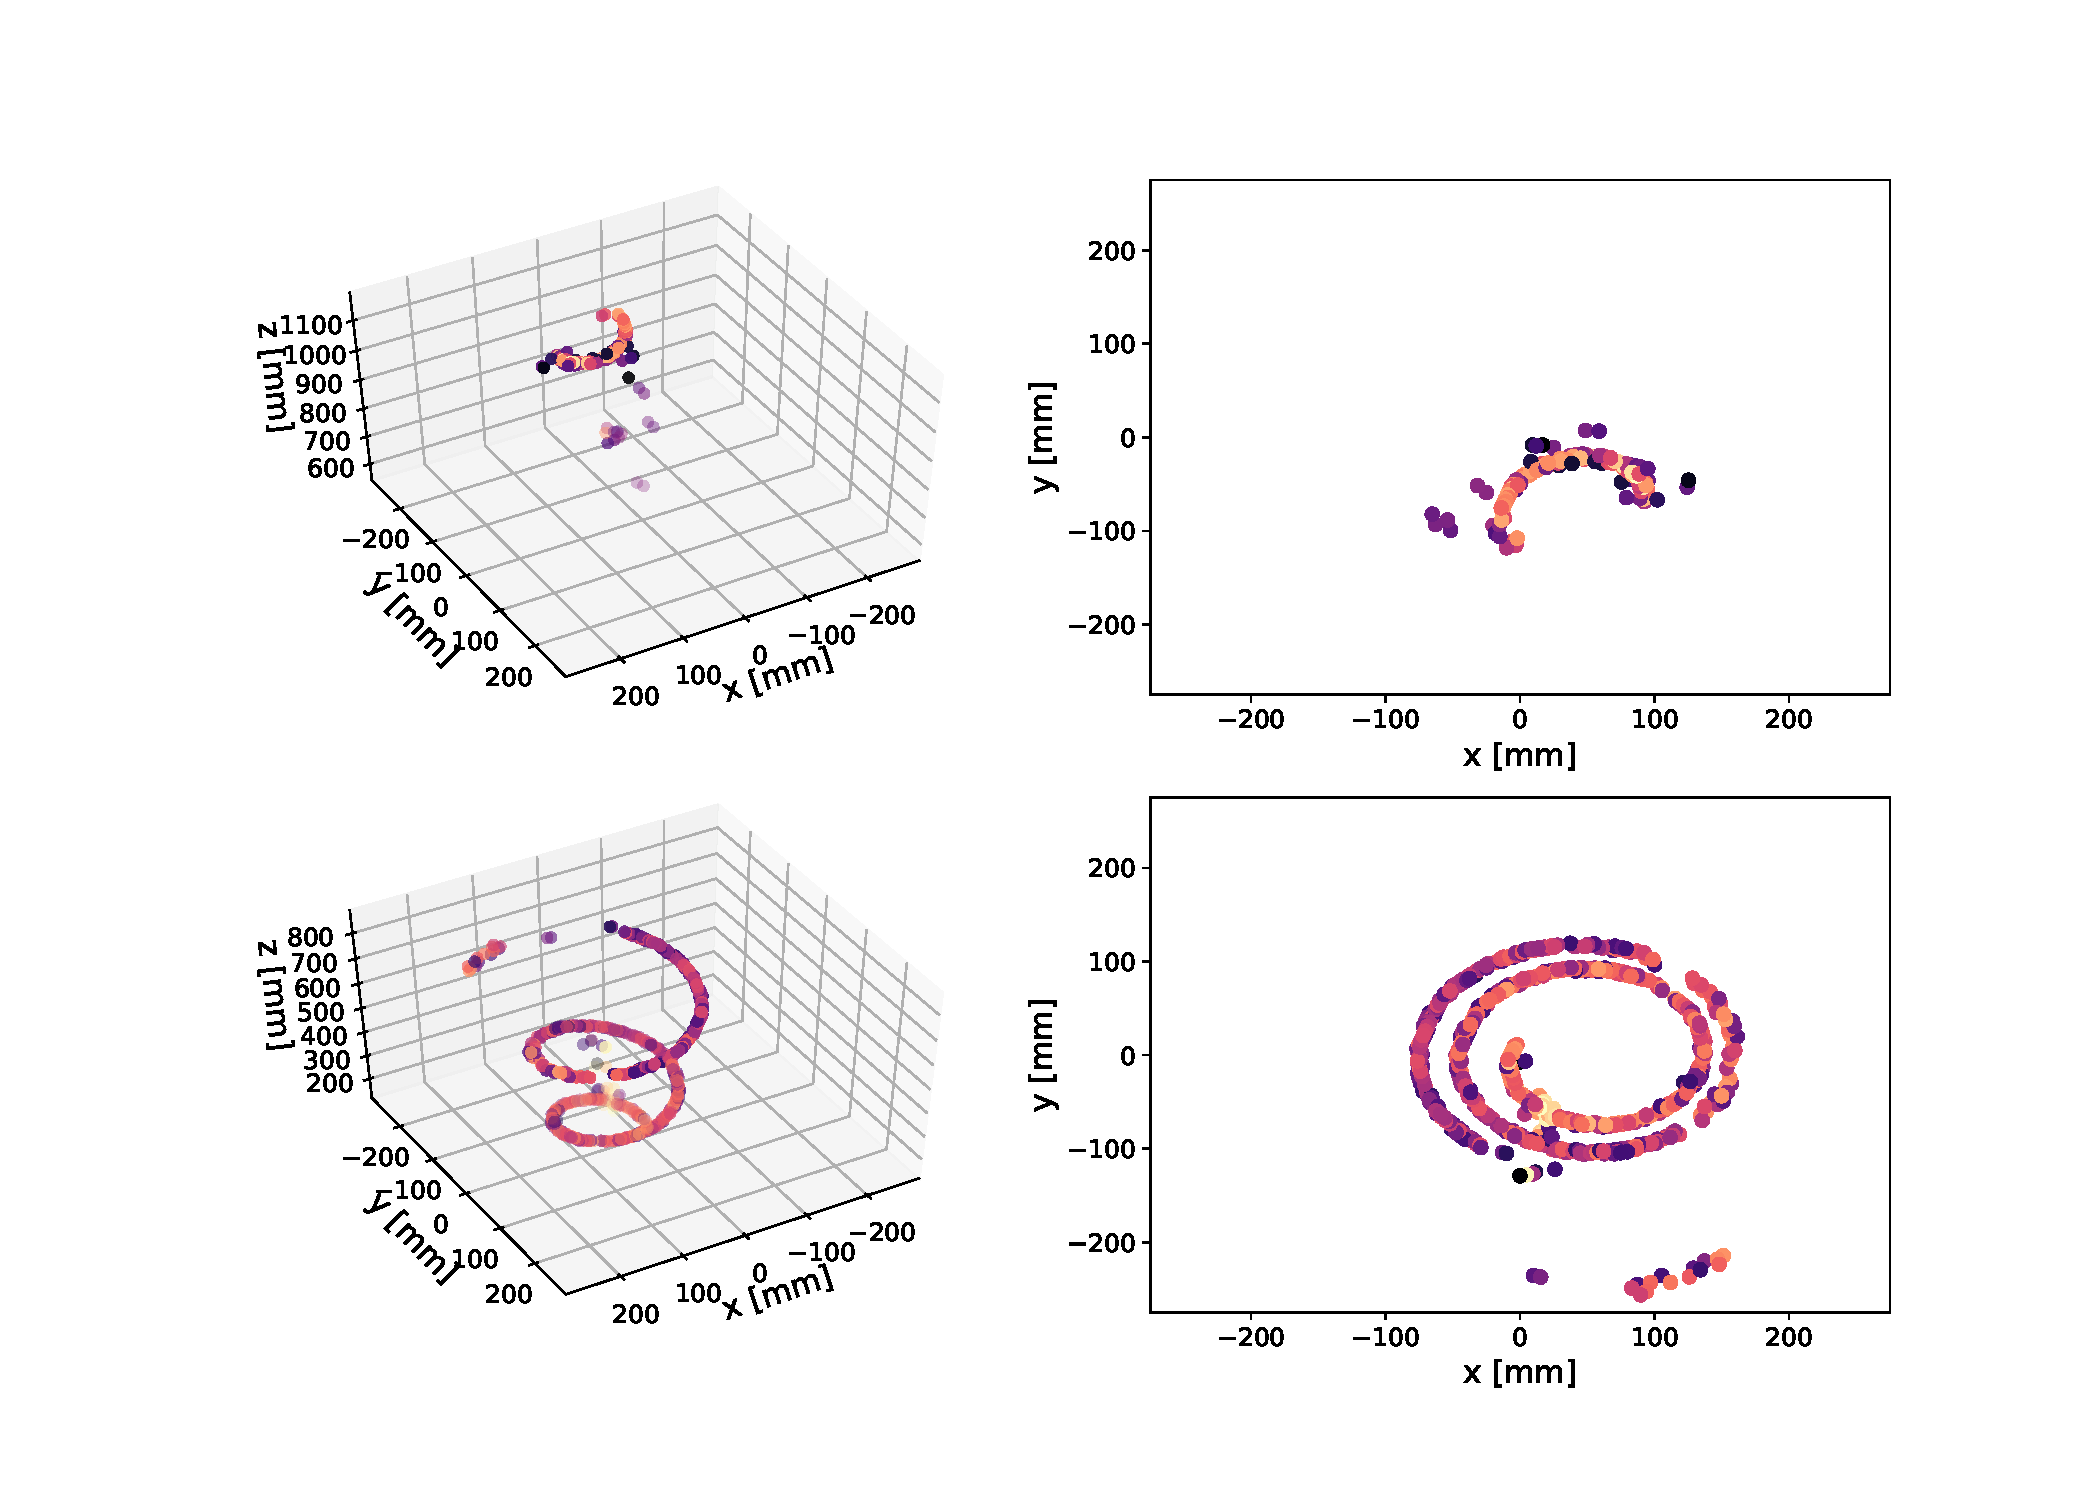
\includegraphics[width=\textwidth]{../plots/display_eventsclean_.pdf}
\caption[Displaying filtered events in 2D and 3D]{Two- and three-dimensional representations of two events from the ${}^{46}Ar$ experiment. Each row is one event in two projections, where the lightness of each point indicates higher charge values. These events have been filtered with a nearest neighbors algorithm and a Hughes' transform, described in section \ref{sec:filtered}}\label{fig:samples_filtered}
\end{figure}
